\section{Section 2}
\label{sec:2}

Citation in text looks like this: \cite{Solcast}. Reference to a figure, equation, section, etc like this: \cref{fig:example-figure}.

\begin{figure}[hb]
    \centering
    \includegraphics[page=4, clip, trim=0.05in 2.2in 7.3in 0.15in, width=1.00\columnwidth]{optimization_demo}
    \caption{PV-Side Power}
    \label{fig:pv-side-power}
\end{figure}

\begin{figure}[hb]
    \centering
    \includegraphics[page=4, clip, trim=0.03in 0.15in 7.3in 2.4in, width=1.00\columnwidth]{optimization_demo}
    \caption{Grid-Side Power}
    \label{fig:grid-side-power}
\end{figure}

\begin{figure}[hb]
    \centering
    % trim=left botm right top
    \includegraphics[page=4, clip, trim=3.5in 2.2in 3.8in 0.15in, width=1.00\columnwidth]{optimization_demo}
    \caption{BSS Energy Stored}
    \label{fig:bss-energy}
\end{figure}

\begin{figure}[hb]
    \centering
    % trim=left botm right top
    \includegraphics[page=4, clip, trim=3.5in 0.15in 3.8in 2.35in, width=1.00\columnwidth]{optimization_demo}
    \caption{BSS Power (Charging \& Discharging)}
    \label{fig:bss-power}
\end{figure}

\begin{figure}[hb]
    \centering
    % trim=left botm right top
    \includegraphics[page=4, clip, trim=7.2in 2.9in 0.1in 0.15in, width=1.00\columnwidth]{optimization_demo}
    \caption{Water Stored}
    \label{fig:water-level}
\end{figure}

\begin{figure}[hb]
    \centering
    % trim=left botm right top
    \includegraphics[page=4, clip, trim=7.2in 1.3in 0.1in 1.7in, width=1.00\columnwidth]{optimization_demo}
    \caption{Water Used}
    \label{fig:water-used}
\end{figure}
